% Course Exam Style
% By: Hamid Zarrabi-Zadeh
% Licenced Under GPL

\documentclass[11pt,a4paper]{article}

\usepackage{graphicx,comment,framed}
\usepackage{amsthm,amssymb,amsmath}
\usepackage{enumitem}
%\usepackage[colorlinks,linkcolor=blue,citecolor=blue]{hyperref}

\usepackage[localise=on, extrafootnotefeatures]{xepersian}
\usepackage[noend]{algpseudocode}


%--------------------- page settings ----------------------

\settextfont[Scale=1.1]{XB Niloofar}
\setdigitfont[Scale=1.1]{XB Niloofar}
%\defpersianfont\sayeh[Scale=1.1]{XB Kayhan Pook}
\addtolength{\textheight}{3.2cm}
\addtolength{\topmargin}{-24mm}
\addtolength{\textwidth}{3cm}
\addtolength{\oddsidemargin}{-1.5cm}

\renewcommand{\labelitemi}{$\small\bullet$}
\renewcommand{\arraystretch}{1.3}


%------------------------ Environments ------------------------------------

\newtheorem{قضیه}{قضیه}
\newtheorem{لم}{لم}
\newtheorem{مشاهده}{مشاهده}
\newtheorem{تعریف}{تعریف}


%-------------------------- Notations ------------------------------------

\newcommand{\IR}{\ensuremath{\mathbb{R}}} 
\newcommand{\IZ}{\ensuremath{\mathbb{Z}}} 
\newcommand{\IN}{\ensuremath{\mathbb{N}}} 
\newcommand{\IS}{\ensuremath{\mathbb{S}}} 
\newcommand{\IC}{\ensuremath{\mathbb{C}}} 
\newcommand{\IB}{\ensuremath{\mathbb{B}}} 

\newcommand{\bR}{\mathbb{R}}
\newcommand{\cB}{\mathcal{B}}
\newcommand{\cO}{\mathcal{O}}
\newcommand{\cG}{\mathcal{G}}
\newcommand{\rM}{\mathrm{M}}
\newcommand{\rC}{\mathrm{C}}
\newcommand{\rV}{\mathrm{V}}

\newcommand{\ceil}[1]{{\left\lceil{#1}\right\rceil}}
\newcommand{\floor}[1]{{\left\lfloor{#1}\right\rfloor}}
\newcommand{\prob}[1]{{\mbox{\tt Pr}[#1]}}
\newcommand{\set}[1]{{\{ #1 \}}}
\newcommand{\seq}[1]{{\left< #1 \right>}}
\newcommand{\provided}{\,|\,}
\newcommand{\poly}{\mbox{\rm poly}}
\newcommand{\polylog}{\mbox{\rm \scriptsize polylog}\,}
\newcommand{\divs}{\ | \ }
\newcommand{\congruent}[1]{\,\overset{#1}{\equiv}\,}

\newcommand{\lee}{\leqslant}
\newcommand{\gee}{\geqslant}
\renewcommand{\leq}{\lee}
\renewcommand{\le}{\lee}
\renewcommand{\geq}{\gee}
\renewcommand{\ge}{\gee}

\newcommand{\REM}[1]{}
\renewcommand{\حذف}{\REM}
\newcommand{\mrbox}[1]{\mbox{\lr{#1}}}

\newcommand{\لر}{\lr}


\newcounter{probcnt}
\newcommand{\مسئله}[1]{\stepcounter{probcnt}\bigskip\bigskip{
 	\large \bf مسئله‌ی \arabic{probcnt}$\mbox{\bf{.}}$ \ #1} \bigskip}

\newcommand{\fqed}[1]{\leavevmode\unskip\nobreak\quad\hspace*{\fill}{\ensuremath{#1}}}

\newenvironment{اثبات}
	{\begin{trivlist}\item[\hskip\labelsep{\em اثبات.}]}
	{\fqed{\square}\end{trivlist}}

\newenvironment{حل}
	{\begin{trivlist}\item[\hskip\labelsep{\bf حل.}]}
	{\fqed{\blacktriangleright}\end{trivlist}}

\ifdefined\hidesols
	\newsavebox{\trashcan} % uncomment the following line to hide solutions
	\renewenvironment{حل}{\begin{latin}\begin{lrbox}{\trashcan}}{\end{lrbox}\end{latin}}
\fi


%------------------------- Header -----------------------------

\newcommand{\سربرگ}[3]{
\parindent=0em

\rightline{
\makebox[5em][c]{
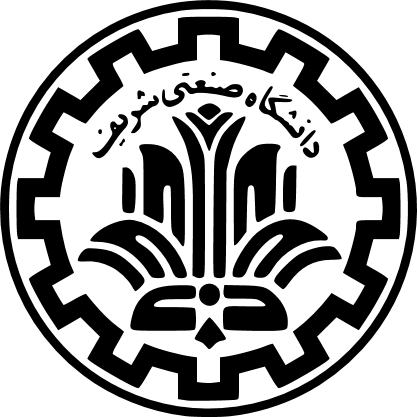
\includegraphics[height=1.5cm]{../commons/sharif.png}
}}
\vspace{-.2em}
{\scriptsize\bf دانشکده‌ی مهندسی کامپیوتر}
\hfill {\small
مدرس:  آبام-بهرامی \  
}\\[-5em]
\leftline{\hfill\large\bf 
ساختمان‌داده‌ها و الگوریتم‌ها
}\\[.2em]
\leftline{\hfill\bf 
نیم‌سال اول ۰۲-۰۳
}\\[1.4em]
\hrule height .12em

\small
\vspace{1mm} 
نام و نام خانوادگی:
\hfill #2 %[2mm]
%شماره‌ی دانش‌جویی:
%\hfill  زمان: #3
%\vspace{1.5mm} 
\hrule height .1em

\vspace{-5.7em} 
\hfill {\large #1} \hfill
\vspace*{4em}
}

\newcommand{\نام‌دانش‌جو}[2]{
\begin{framed}
نام دانش‌جو: #1\hfill شماره‌ی دانش‌جویی: #2
\end{framed}
}

\pagestyle{empty} 



\شروع{نوشتار}

\سربرگ{آزمون میان‌ترم اول}{۹ آذر ۱۴۰۲}{۱۵۰ دقیقه}
\medskip


\مسئله{پشتگان پرتوان} [۲۵ نمره]

\شروع{شمارش}[label=(\alph*)]
\فقره نشان دهید می‌توان با استفاده از یک آرایه و حافظه‌ی اضافی $O(1)$ دو پشته را پیاده‌سازی کرد. (توجه کنید که زمانی یک پشته نمی‌تواند عمل Push را انجام دهد که کل آرایه پر شده باشد) (۱۰ نمره)
\فقره فرض کنید در صورتی که آرایه‌ی ما پر شود، آرایه‌ای با  سایز $ 2n $ گرفته و عناصر آرایه‌ی اولیه را در آرایه‌ی دوم کپی می‌کنیم. ضمن مشخص کردن ترتیب کپی، هزینه‌ی سرکشن اعمال $ Push $ و $ Pop $ را  محاسبه کنید. (۱۵ نمره)
\پایان{شمارش}
\مسئله{انتخاب تصادفی}[۲۰ نمره]

الگوریتمی را در نظر بگیرید که ورودی $ a_1, \dots, a_n $ شامل $ n $ عدد مجزا را به ترتیب داده شده می‌خواند و هنگام خواندن $ a_i $ مقدار متغیر $ x $ را به احتمال $ 1/i $ برابر $ a_i $ قرار می‌دهد. الگوریتم در پایان مقدار $ x $ را به عنوان خروجی گزاری می‌کند. با چه احتمالی خروچی الگوریتم $ a_i $ است؟


\مسئله{رابطه‌ی بازگشتی}[۲۰ نمره]

رابطه‌ی بازگشتی زیر را در نظر بگیرید:
$$T(n) = T(an) + T(bn) + \mathcal{O}(n)$$
\شروع{شمارش}[label=(\alph*)]
\فقره ثابت کنید اگر $ a + b < 1 $ آنگاه $ T(n) $ از $ \mathcal{O}(n) $ است.
\فقره ثابت کنید اگر $ a + b = 1 $ آنگاه $ T(n) $ از $ \mathcal{O}(n\log{n}) $ است.
\پایان{شمارش}




\مسئله{ابر هرم بیشینه}[۲۵ نمره]

یک هرم چند وجهی یا
 $ d $-هرم
 یک درخت $ d $ تایی کامل است (بجز حداکثر یک عنصر یا یک فرزند) که برگ‌های سطر آخر آن از سمت چپ چیده شده‌اند و کلید هر عنصر بزرگ‌تر یا مساوی کلید همه‌ی نوادگانش است. در این مسئله قصد داریم اعدادی که در آرایه‌ای به طول $ n $ ذخیره شده‌اند را به یک $ d $-هرم تبدیل کنیم که در همان آرایه نگهداری شود.

\شروع{شمارش}[label=(\alph*)]
\فقره اگر آرایه‌ی داده شده خاصیت $ d $-هرم را داشته باشد، فرزندان و پدر گره‌ای که در اندیس  $ i $ ذخیره شده است در چه خانه‌هایی ذخیره می‌شوند؟ (۵ نمره)
\فقره الگوریتم ساخت این هرم را بنویسید. (۱۰ نمره)
\فقره ضمن نوشتن الگوریتم حذف بزرگترین کلید یا همان \lr{Extract-Max} زمان اجرای آن محاسبه و درستی آن را ثابت کنید. (۱۰ نمره)
\پایان{شمارش}

\مسئله{بازسازی}[۲۰ نمره]

در این مسئله قصد داریم بازسازی درخت‌های دودویی کامل از روی پیمایش‌های پیش‌وندی و پس‌وندی بررسی کنیم.
\شروع{شمارش}[label=(\alph*)]
\فقره فرض کنید پیشمایش پیش‌وندی و پس‌وندی یک درخت به شرح زیر است. آیا می‌توانید این درخت را بسازید؟
\begin{latin}
$ Preorder:\ abehdfilcjmnk \qquad \qquad Postorder:\ edfhblmnjkcia $
\end{latin}
\فقره آیا در حالت کلی می‌توان با پیمایش‌های پیش‌وندی و پس‌وندی یک درخت دودویی کامل را ساخت؟ در صورتی که پاسخ‌تان مثبت است یک الگوریتم به این منظور ارائه دهید و در غیر این صورت یک مثال نقض بزنید.

\پایان{شمارش}





\پایان{نوشتار}
